\documentclass[11pt]{article}
\usepackage[letterpaper]{geometry}
\usepackage{times}
\usepackage{verbatim}
\usepackage{graphicx}
\usepackage{float}
\usepackage{fullwidth}
\usepackage{amsmath}
\usepackage{amssymb}
\usepackage{hyperref}
\graphicspath{{Images/}}
\title{ENGR-241 Transfer Function Lab}
\author{Jeremy Munson, Lauren Speirs \& Andrew Henrikson}
\geometry{top=.8in, bottom=.8in, left=.8in, right=.8in}

\setlength{\parindent}{0em}
\setlength{\parskip}{.5em}
\begin{document}
	\maketitle
	\subsection*{Overview}
	For this lab we calculated the transfer function then built the required circuit from the lab guidelines. We then calculated the voltage across the capacitor and compared our results from our circuits output to the oscilloscope. We then built the circuit using Orcad and analyzed the ciruit using the Laplace function in Pspice and compared its output to our previous results.
		\subsection*{Circuit Diagrams}
			\begin{figure}[H]
			\centering
			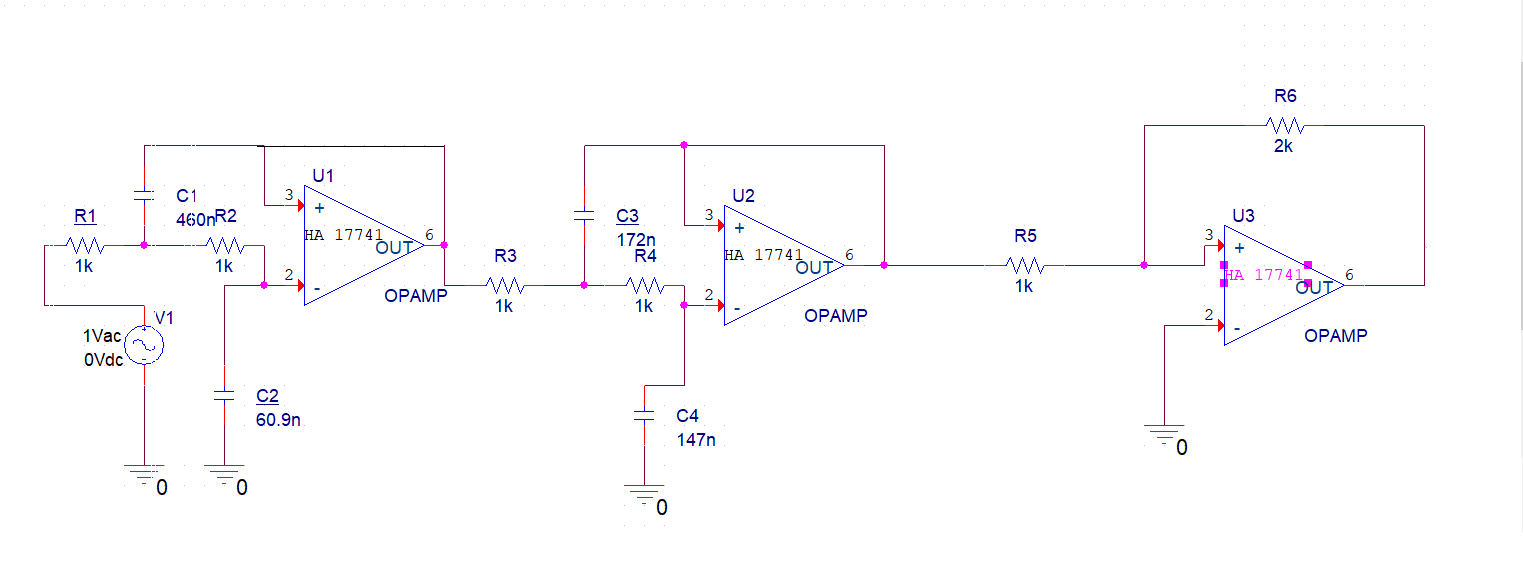
\includegraphics[width=5in]{images/diagram.png}
		\end{figure}
		
		Our suggested values and measured values for our components used are shown in the table below. The percent error is also listed.
		\begin{table}[H]
		\def\arraystretch{1.2}%
		\begin{tabular}{|l|l|l|l|}
			\hline
			Components       	& Suggested 		& Measured      	&\% Diff	\\ \hline
			Resistor 1   		& $1 k\Omega$		& $0.998 k\Omega$   & 2\%	     \\ \hline	
			Resistor 2			& $240 \Omega$		& $241 \Omega$      & 0.4\%       \\ \hline
			Inductor			& $220\mu H$		& $199\mu H$		& 10.6\%		\\ \hline
			Capacitor			& $1 \mu F$			& $0.95 \mu F$		&5.3\%		\\ \hline
		\end{tabular}
	\end{table}
	

	
	\subsection*{Calculations}
	
	\subsection*{Procedure}
	The circuit was simple to construct using the breadboard. Aside from constructing the circuit as normal, we used the LCR meter to select a capacitor and an inductor that were as close to the exact values specified as possible. In order to get the desired value of L, we used two inductors in series. After constructing the circuit, measurements were taken in the usual manner using the oscilloscope. The circuits output is shown below.
		\begin{figure}[H]
		\centering
		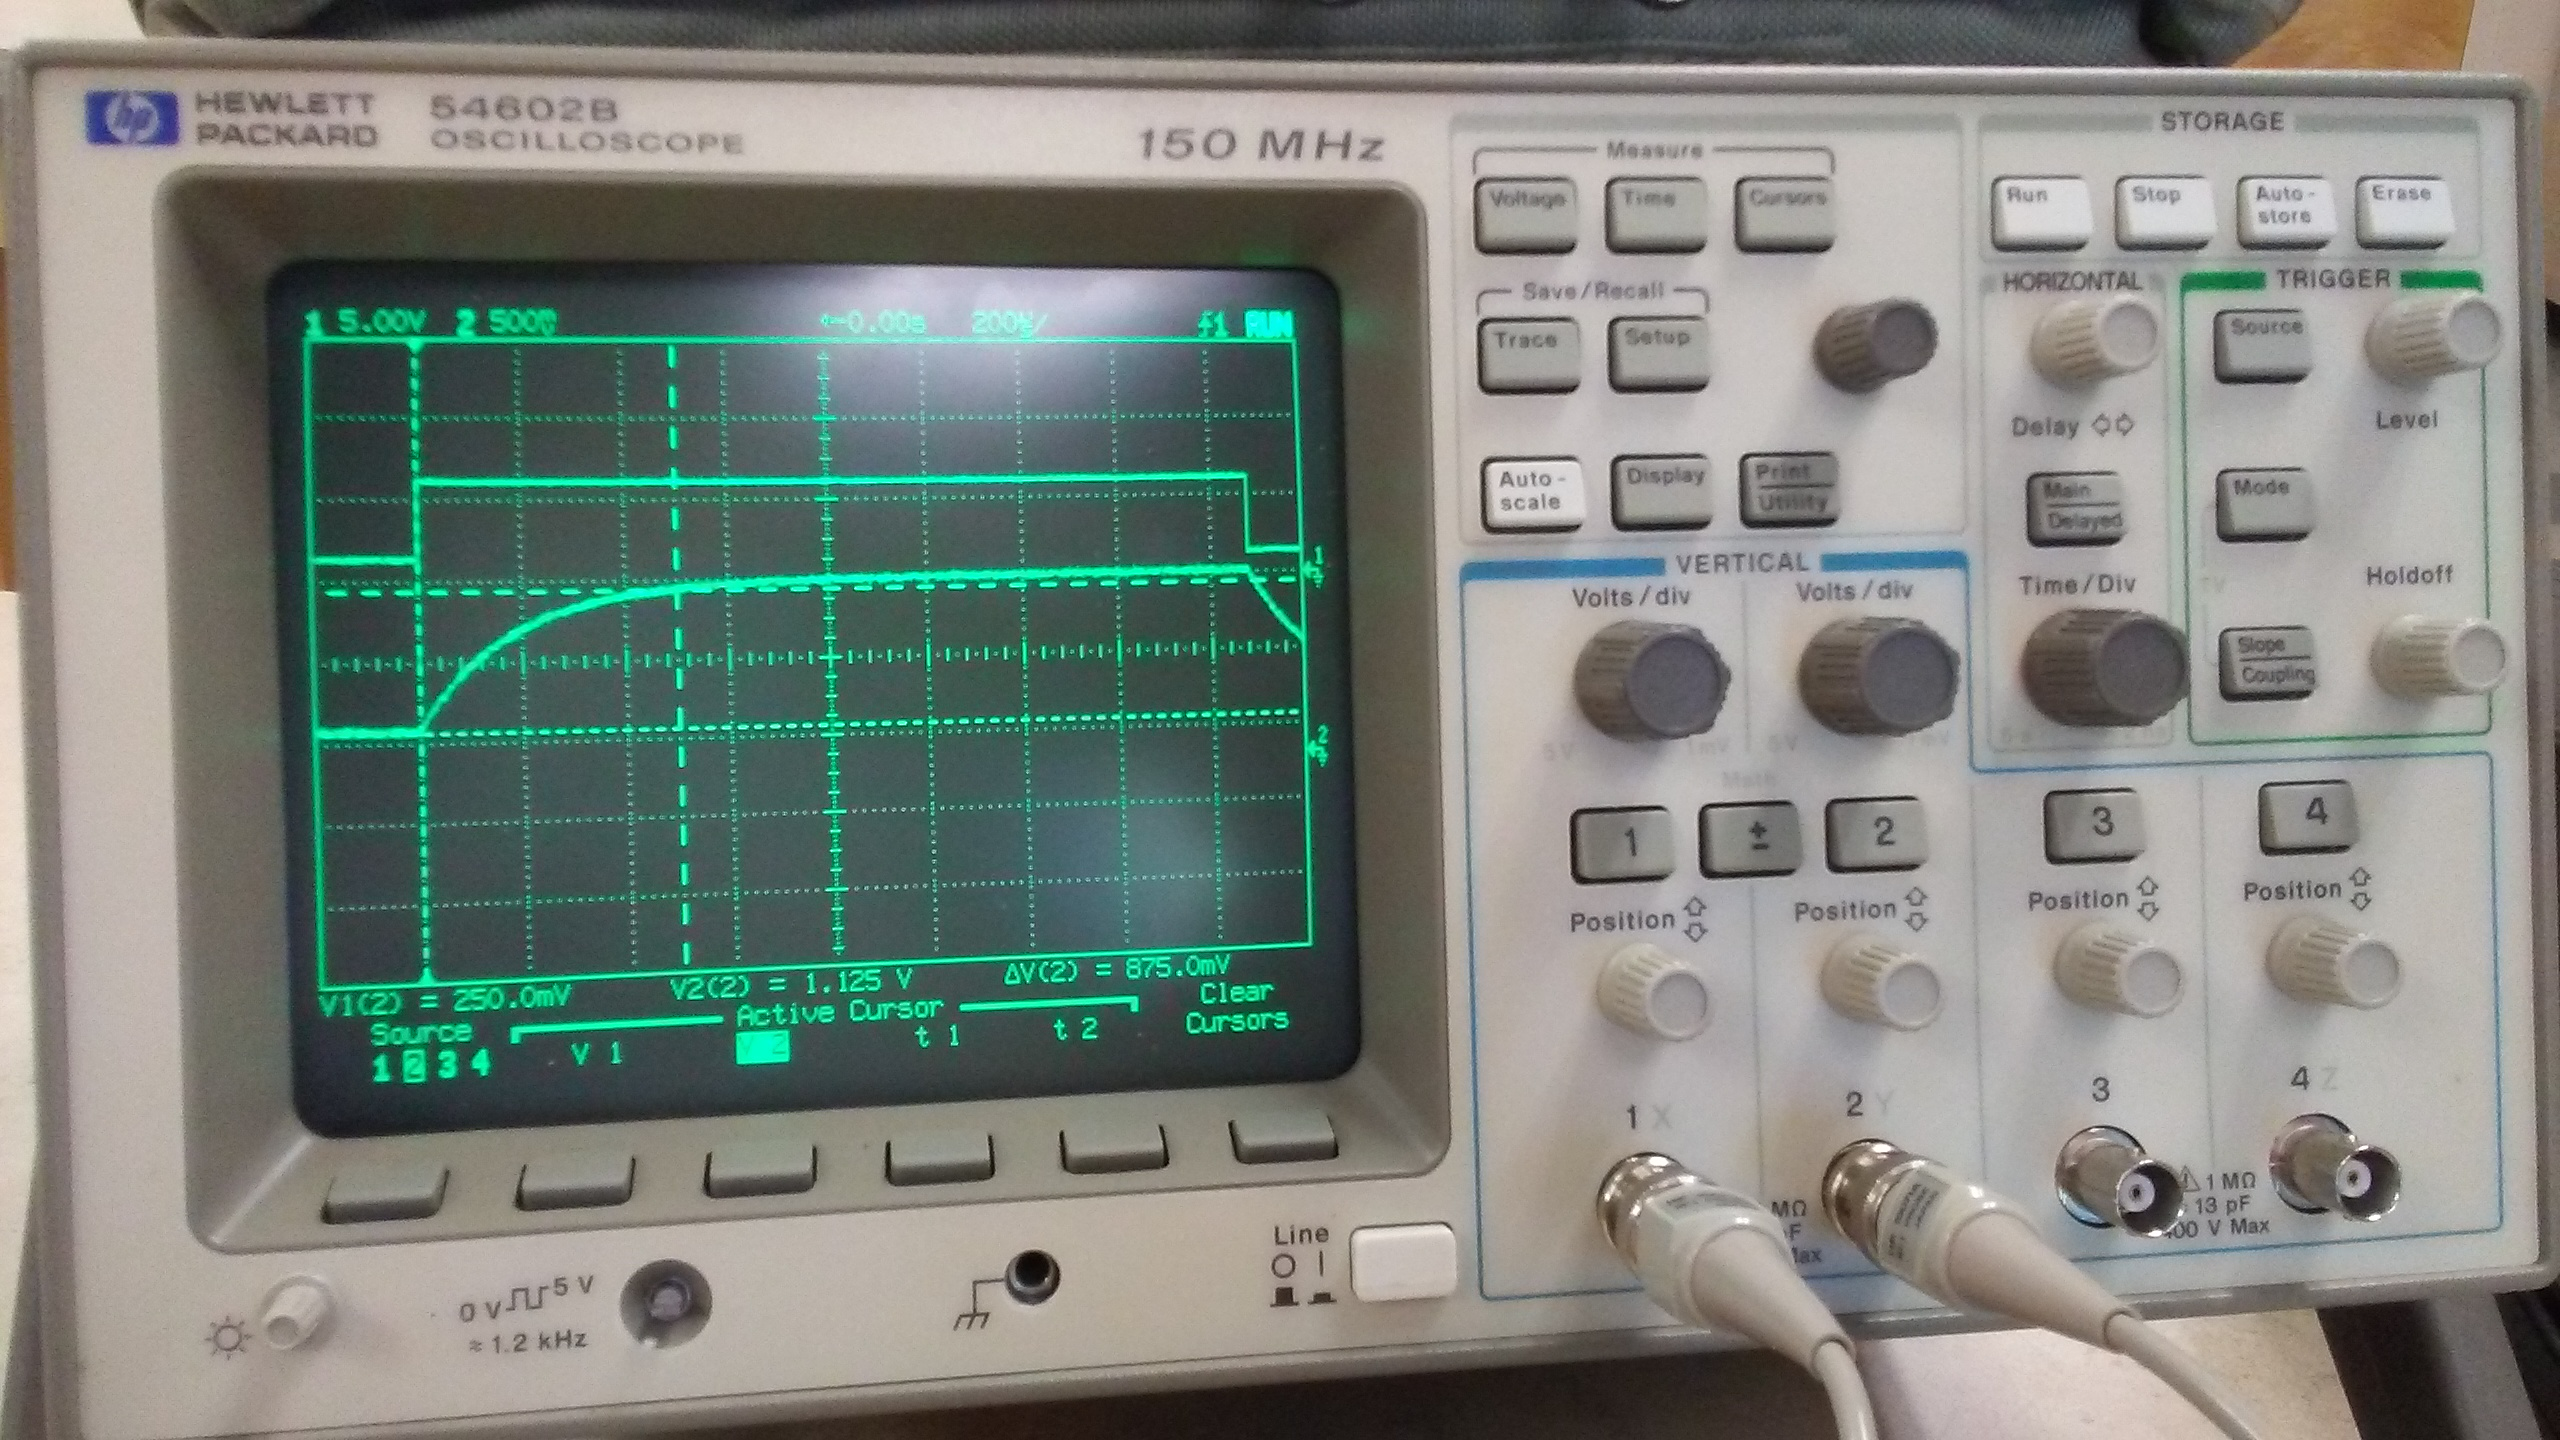
\includegraphics[width=5in]{images/oscilloscope_transfer.jpg}
		\end{figure}
	We then performed simulations of the same circuit in Orcad. The graph below is the output from the simulation.
		\begin{figure}[H]
		\centering
		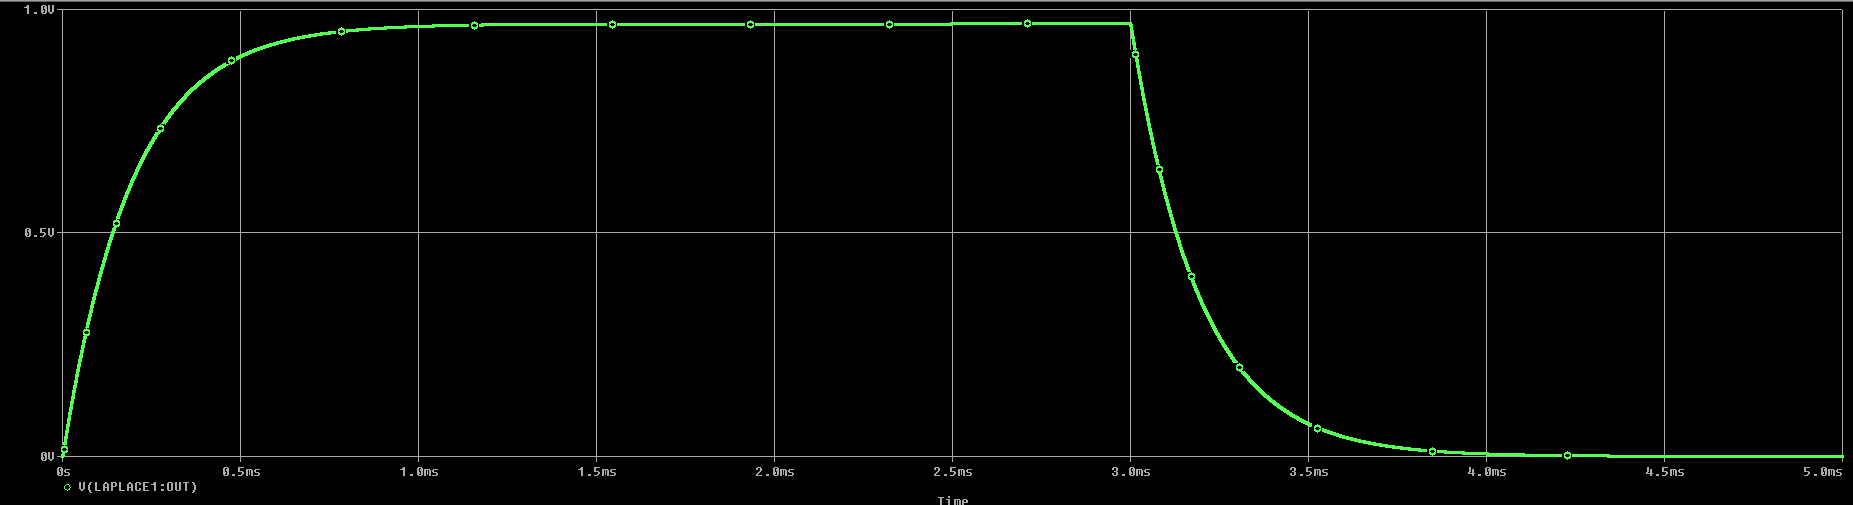
\includegraphics[width=6in]{images/simulated_curve.png}
		\end{figure}

	We subsequently used the Laplace feature in Orcad to verify our calculations. 
	
		\begin{figure}[H]
		\centering
		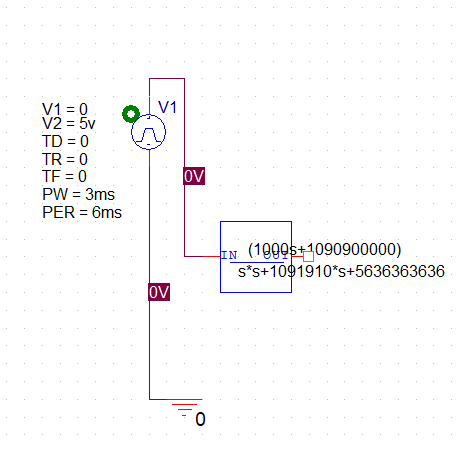
\includegraphics[width=5in]{images/simulation_schematic.png}
		\end{figure}
		\begin{figure}[H]
		\centering
		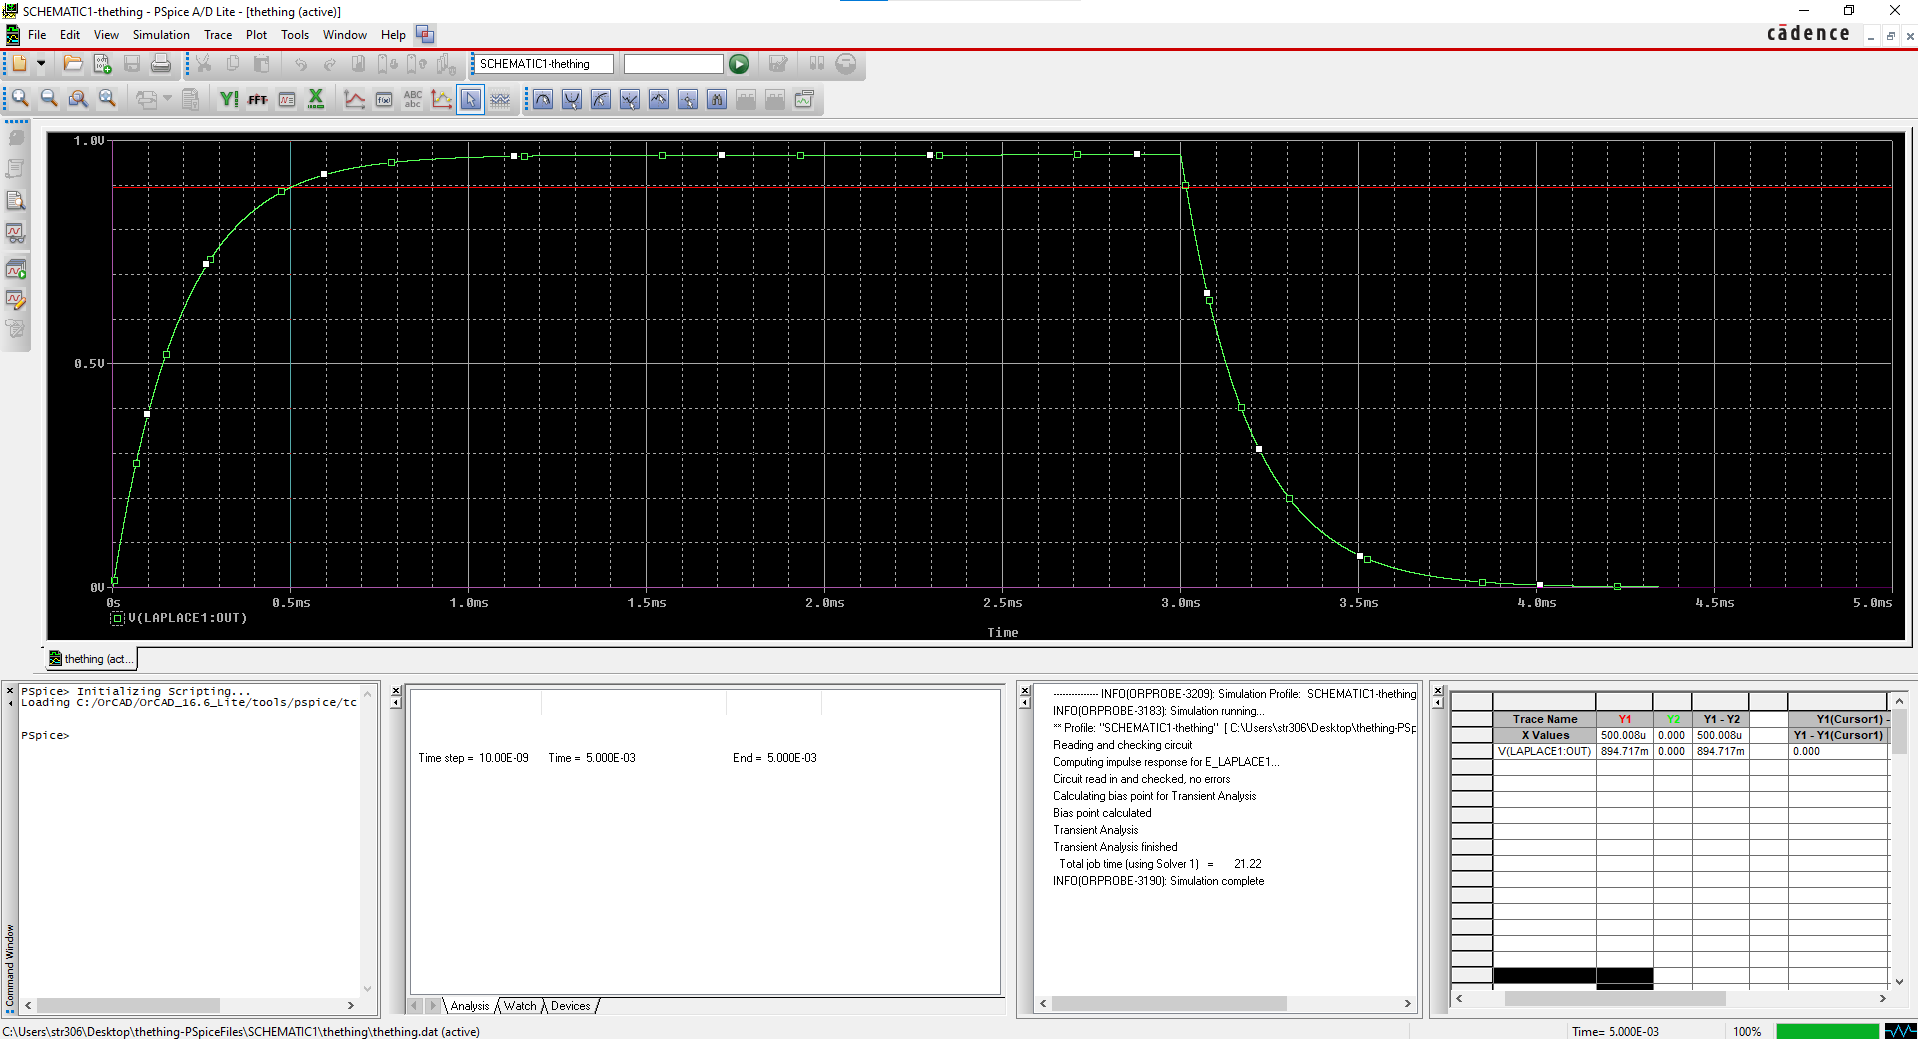
\includegraphics[width=5in]{images/laplace_part.png}
		\end{figure}
	

	\subsection*{Error Analysis}
	
	\subsection*{Conclusion}
	The lab was performed without issue. We were able to successfully calculate, simulate and build the circuit. Our results were excellent with minimal error. 
	
	
\end{document}
